\section{Cahier des charges}
    \label{sec:cahier}
    % Preciser utilisateur
    % Connais deja concept arbre d'attaque
    % Responsable securite d'une entite
    % Preciser des l'intro

    % Structure reflete niveau importance

    Comme indiqué dans la section \ref{sec:objectifs}, notre principal objectif est de réaliser un logiciel pouvant assister l'expert en sécurité d'une entreprise. Il devra pouvoir réaliser facilement l'analyse de son système\footnote{La nature du dit système pouvant être très vaste, allant d'une base de donnée à un distributeur de billet, en passant par une prison haute sécurité.}, en utilisant les arbres d'attaque et de défense décrits dans la section \ref{sec:etat_art}.

    Plusieurs fonctionnalités peuvent être rajoutées afin de faciliter l'analyse:
    \begin{itemize}
        \item Trouver le chemin d'attaque optimal en fonction d'une fonction de synthèse, qui utilisera plusieurs types de valuation. Nous détaillerons cette fonctionnalités dans la section \ref{sec:fct_synth}
        \item Filtrer l'arbre en fonction d'une fourchette de critères. Voir section \ref{sec:filtre}.
        \item L'utilisation de modèles (d'arbres) généraux que l'utilisateur pourra ensuite modifier en fonction de sa situation. Voir section \ref{sec:modele}
    \end{itemize}

    De plus, l'édition des arbres avec ADTool peut être améliorée, afin d'être plus souple et plus pratique. Nous détaillerons nos futures améliorations dans la section \ref{sec:adtoolpp}.

    Nous décrirons ensuite la forme et l'architecture de notre logiciel dans la section \ref{sec:archi}.

    \subsection{Fonction de synthèse et chemin optimal}
        \label{sec:fct_synth}


    \subsection{Filtre à critères}
        \label{sec:filtre}


    \subsection{Modèles généraux}
        \label{sec:modele}


    \subsection{Amélioration d'ADTool}
        \label{sec:adtoolpp}
    

    \subsection{Architecture}
        \label{sec:archi}

        \begin{figure}
            \begin{center}
                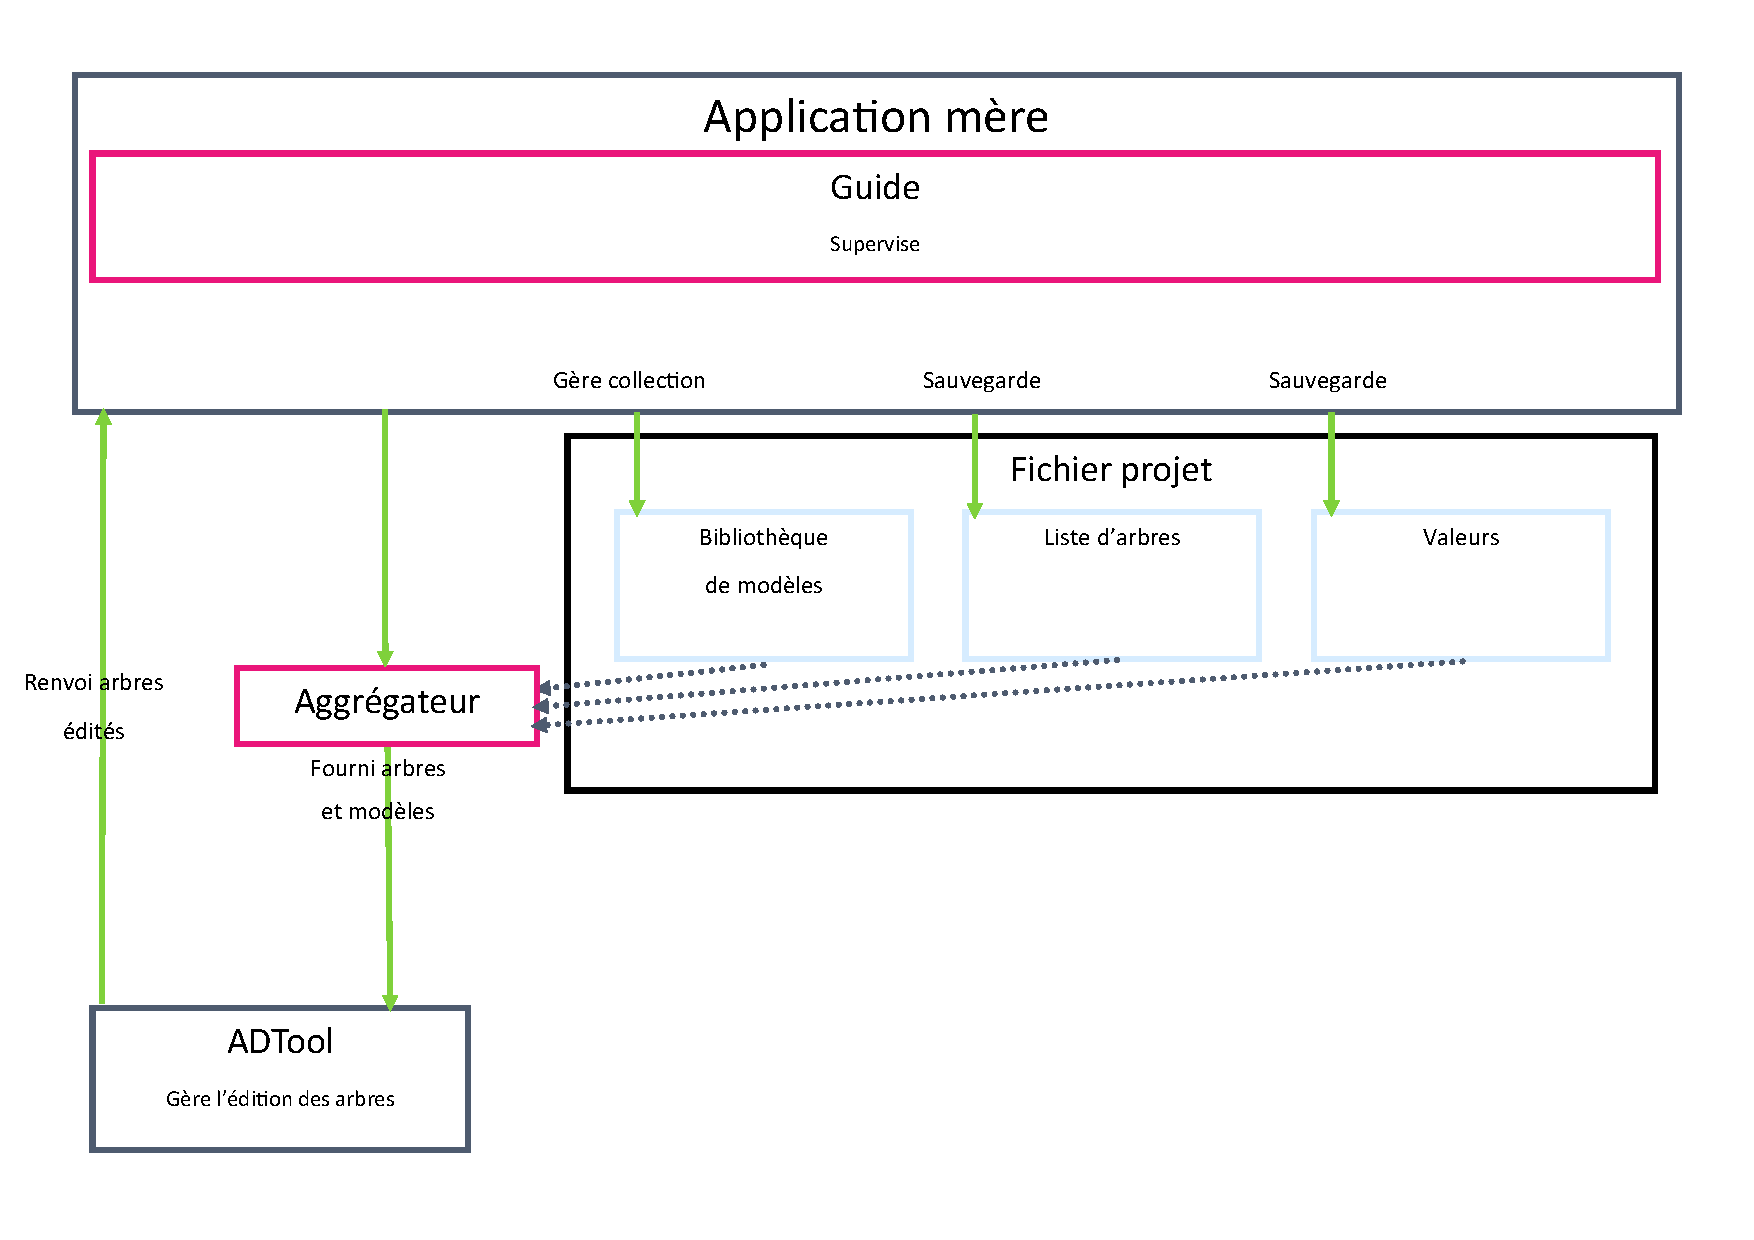
\includegraphics[width=1\textwidth]{figure/archi.pdf}
            \end{center}
            \caption{Différents composants interviendront pour éditer le fichier projet.}
            \label{fig:archi}
        \end{figure}


    \subsection{Synthèse}
        \label{sec:cahier_synthese}